% Testing
    %Overview with table
    % Simulator sub
        %vehicle subsub
        %gnss subsub
        %full system subsub
    % UBX log sub
    % serial device sub
    % IMC log sub

%   Simulators for testing
%       + SITL, JSBSim, Flightgear, Simple GNSS

To verify that the whole system was working as intended different methods were used, listed in table \ref{tab:testing}. The EKF alone was first tested with the simulator described in section \ref{sec:imp:simulator}. Next, the RTKLIB task was tested by configuring it to read real world measurements from a UBX-log file. The system was then tested on real world GNSS data by connecting a GNSS receiver over USB. Finally, the full system was tested and tuned by a log of IMC messages gathered from a test run of the hardware package.\\
\label{sec:imp:testing}
\begin{table}[!htbp]
    \centering
    \begin{tabular}{|l|l|}\hline
         \textbf{Testing method}& \textbf{Tested system}\\\hline
         Simulator              & EKF only\\
         UBX log                & RTKLIB and EKF (without IMU)\\
         Stationary receiver    & Reading and configuration of serial device\\
         IMC log                & The full system\\\hline
    \end{tabular}
    \caption{Course of testing}
    \label{tab:testing}
\end{table}
    
\subsection{Simulator}
\label{sec:imp:simulator}
    \subsubsection{Vehicle simulation}
        \todo{write about vehicle simulation}
        With software in the loop (SITL), ardupilot can be run without any hardware. The vehicle is simulated through a flight dynamics model (FDM) which communicates with a flight simulator. The flight simulator simulates measurements and dispatches these to ardupilot. Ardupilot is configured to work with the FDM JSBsim. It is cross platform and contains models for a range of different vehicles, although this implementation simply uses the default model of the Rascal110 RC plane. \todo{is flightgear the default simulator?}\\
    
        \todo{
            Questions: 
            What is the default alternative to FG?
            What is the role of ardupilot in the simulator?
            Why is there a direct connection between FG and DUNE?
            Why does FG provide a better resolution for IMU?
            Including the FG task send measurements directly to AP-task?
            Is the precision lowered when it goes through AP?
            Is JSBsim the default FDM?
            Does Mavproxy and Neptus communicate?
        }
        \todo{Hva var alternativet til flightgear?}
        %\paragraph{JSBsim}
        %http://jsbsim.sourceforge.net/
        %http://wiki.flightgear.org/JSBSim
        %Bare bones system model that runs on multiple OS's
        %"Flight dynamics model"
        %is a cross platform flight dynamics model. It supports vehicles of many different kinds
    
    %\paragraph{Flightgear}
        %http://wiki.flightgear.org/Flightgear
        %Built on top of jsbsim. Adds a visual interface, cross platform
        %Flight simulator 
%        is a flight simulator running on top of a flight dynamics model, such as JSBsim. It has been used instead of the native ardupilot simulator because of its better IMU measurement precision.
    
%\subsection{ArduPilot Software In The Loop}
    %http://ardupilot.github.io/MAVProxy/html/index.html
    %Neptus, mavproxy, flightgear, gnss / rtklib playback file
%    With software in the loop (SITL), ardupilot can be run without any hardware. 

    \subsubsection{GNSS}
        A simple GNSS simulator has been implemented in DUNE. The focus of the simulator is to provide pseudorange and doppler measurements to a receiver, and as such no ephemeris calculations are made for the simulated satellite positions or velocity. For simplicity the satellites are kept stationary with zero velocity. Positions are taken from a snapshot of visible GPS satellites in the Trondheim area at 13:00 the 13th of November 2018. A visibility plot shows the satellites with respect to elevation angle and azimuth in figure \ref{fig:visplot}.\\

        %Constellation of six stationary satellites with no noise or bias
        %Subscribes to ExternalNavData
        \begin{figure}[!htbp]
            \centering
            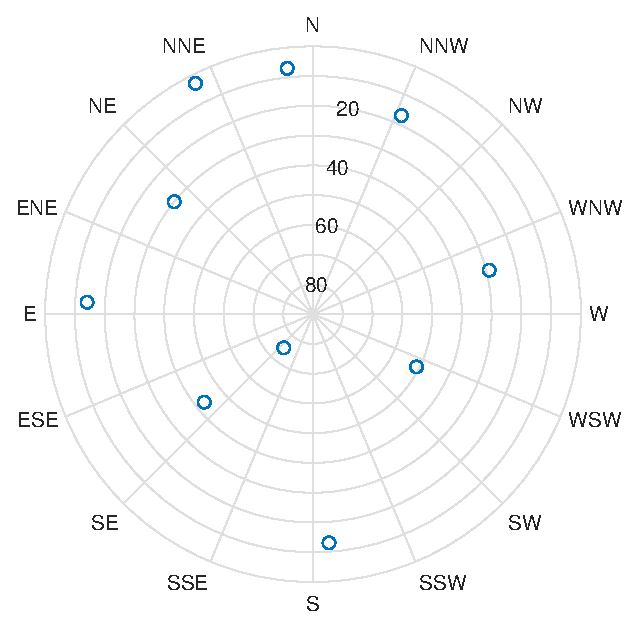
\includegraphics[scale=0.7]{Implementation/Images/visibilityplot.eps}
            \caption{Visibility plot of the satellites in the simulator from Trondheim. The user position is in the middle, while the dots denote satellites above the horizon. The distance between user and satellites in the plot is the given by the elevation angle. The angle from the north axis is the azimuth.}
            \label{fig:visplot}
        \end{figure}

    Each satellite of the simulator runs as a separate task on the system. The output of the tasks comes in the form of the IMC message RawGNSSdata, containing satellite position and range and doppler shift measurements. The input is another IMC message, ExternalNavData, containing the true state of the system, dispatched by the ardupilot task. As all the satellites in the constellation run as separate tasks, the true state will be received at the same time for all satellites. In other words, the satellites dispatch messages separately while sharing inputs. As a result, GNSS-messages will be dispatched approximately simultaneously, resulting in messages being sent in \textit{bursts}, resulting in an excessively small time step between measurements. This is not ideal for a discretized system and should be handled. Distinct delays between the satellite tasks are therefore introduced, which spread the dispatching of GNSS messages evenly. Another option would be to buffer the GNSS messages at the integration filter and run all measurements together, but this introduces an unnecessary layer of complexity for the filter. \\
    \todo{forsinkelse i posisjon mellom simulator og filter (noen pseudoranges blir feil/utdatert)}
    \todo{PX BBB 20 ms delay?}
    \todo{Perfect measurements}
    
    \subsubsection{Full simulator system}
        %SIM_VEHICLE: "mavproxy.py" "--master" "tcp:127.0.0.1:5760" "--sitl" "127.0.0.1:5501" "--out"  "127.0.0.1:14550" "--out" "127.0.0.1:14551" "--map" "--console"
        %flightgear: 5503
        %ntnu-x8-001 on AP serial 2
        %dune task: tcp:5760
        %Neptus and mavproxy
        \todo{write about full simulator}
        \todo{Dune bridges the connection between Neptus and ArduPilot by relaying setpoints and states}
        Neptus is configured to interface with Ardupilot and can be used to control the simulated vehicle. Not only does this provide the operator with a visual interface for executing maneuvers, but it also offers extensive plotting functionality of messages from the IMC bus shared with DUNE, which is helpful for debugging. DUNE is also configured to run the FlighGear task that offers a IMU measurements with a higher resolution than those received from arduplane. A block diagram of the full simulator is shown in figure \ref{fig:sim-diag}
        
        \begin{figure}
            \centering
            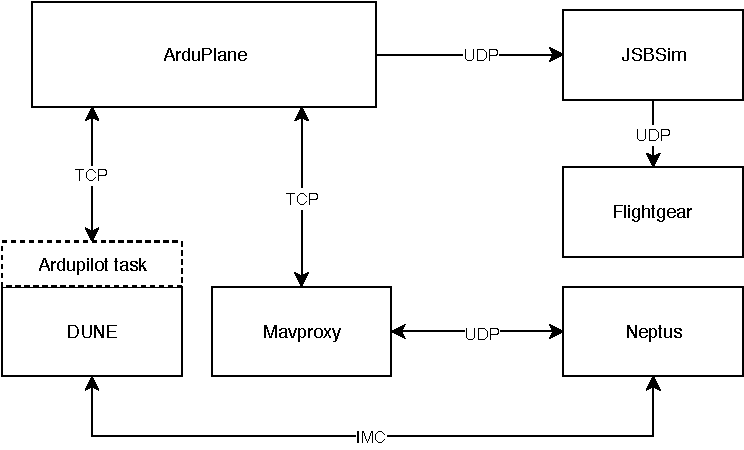
\includegraphics[scale=0.8]{Images/Simulator.pdf}
            \caption{Simulator block diagram}
            \label{fig:sim-diag}
        \end{figure}
        
    \todo{Lea-m8t connected to computer. U-center config. RTKLIB. }
    \subsection{UBX log}
        \label{sec:rtklib-ubx-log}
        %The rtklib task can log real world data.
        To test both the RTKLIB and EKF tasks together, reading GNSS measurements from a log file is beneficial. Testing can begin immediately after updating code as there is no need to wait for signal acquisition, nor for the ephemeris to download. Additionally, the same log can easily be run with external software, such as RTKLIB, to provide a navigation solution that can be kept as a reference. It is also beneficial as a verification that the integration filter works as intended on real world, noisy data. RTKLIB supports several input protocols, one of which is, as mentioned, the ubx log format. For the dune task equivalent this functionality was included. However, in RTKLIB, this is not designed to work in real time, in that log files are handled as fast as possible. A buffer for storing the measurements of the logfile was therefore added, periodically pushing its contents to the IMC bus according to the original time stamps of each measurement.
    
    \subsection{Serial device}
        As the system was tested on a computer, a ublox LEA-M8T multi-GNSS receiver can easily be connected by USB, pictured in figure \ref{fig:lea-m8t}. The receiver is configured to output raw measurements by the RTKLIB task, specified by a CMD file. This tests the ability to change the input source based on a configuration file, configuration of a connected serial device and the reading of serial data. The receiver output is \textit{message based}, meaning that it can output several distinct message types with different information. U-center lists the message types being output by a connected receiver, and can therefore be used to verify the configuration.
        
        \begin{figure}[!htbp]
            \centering
            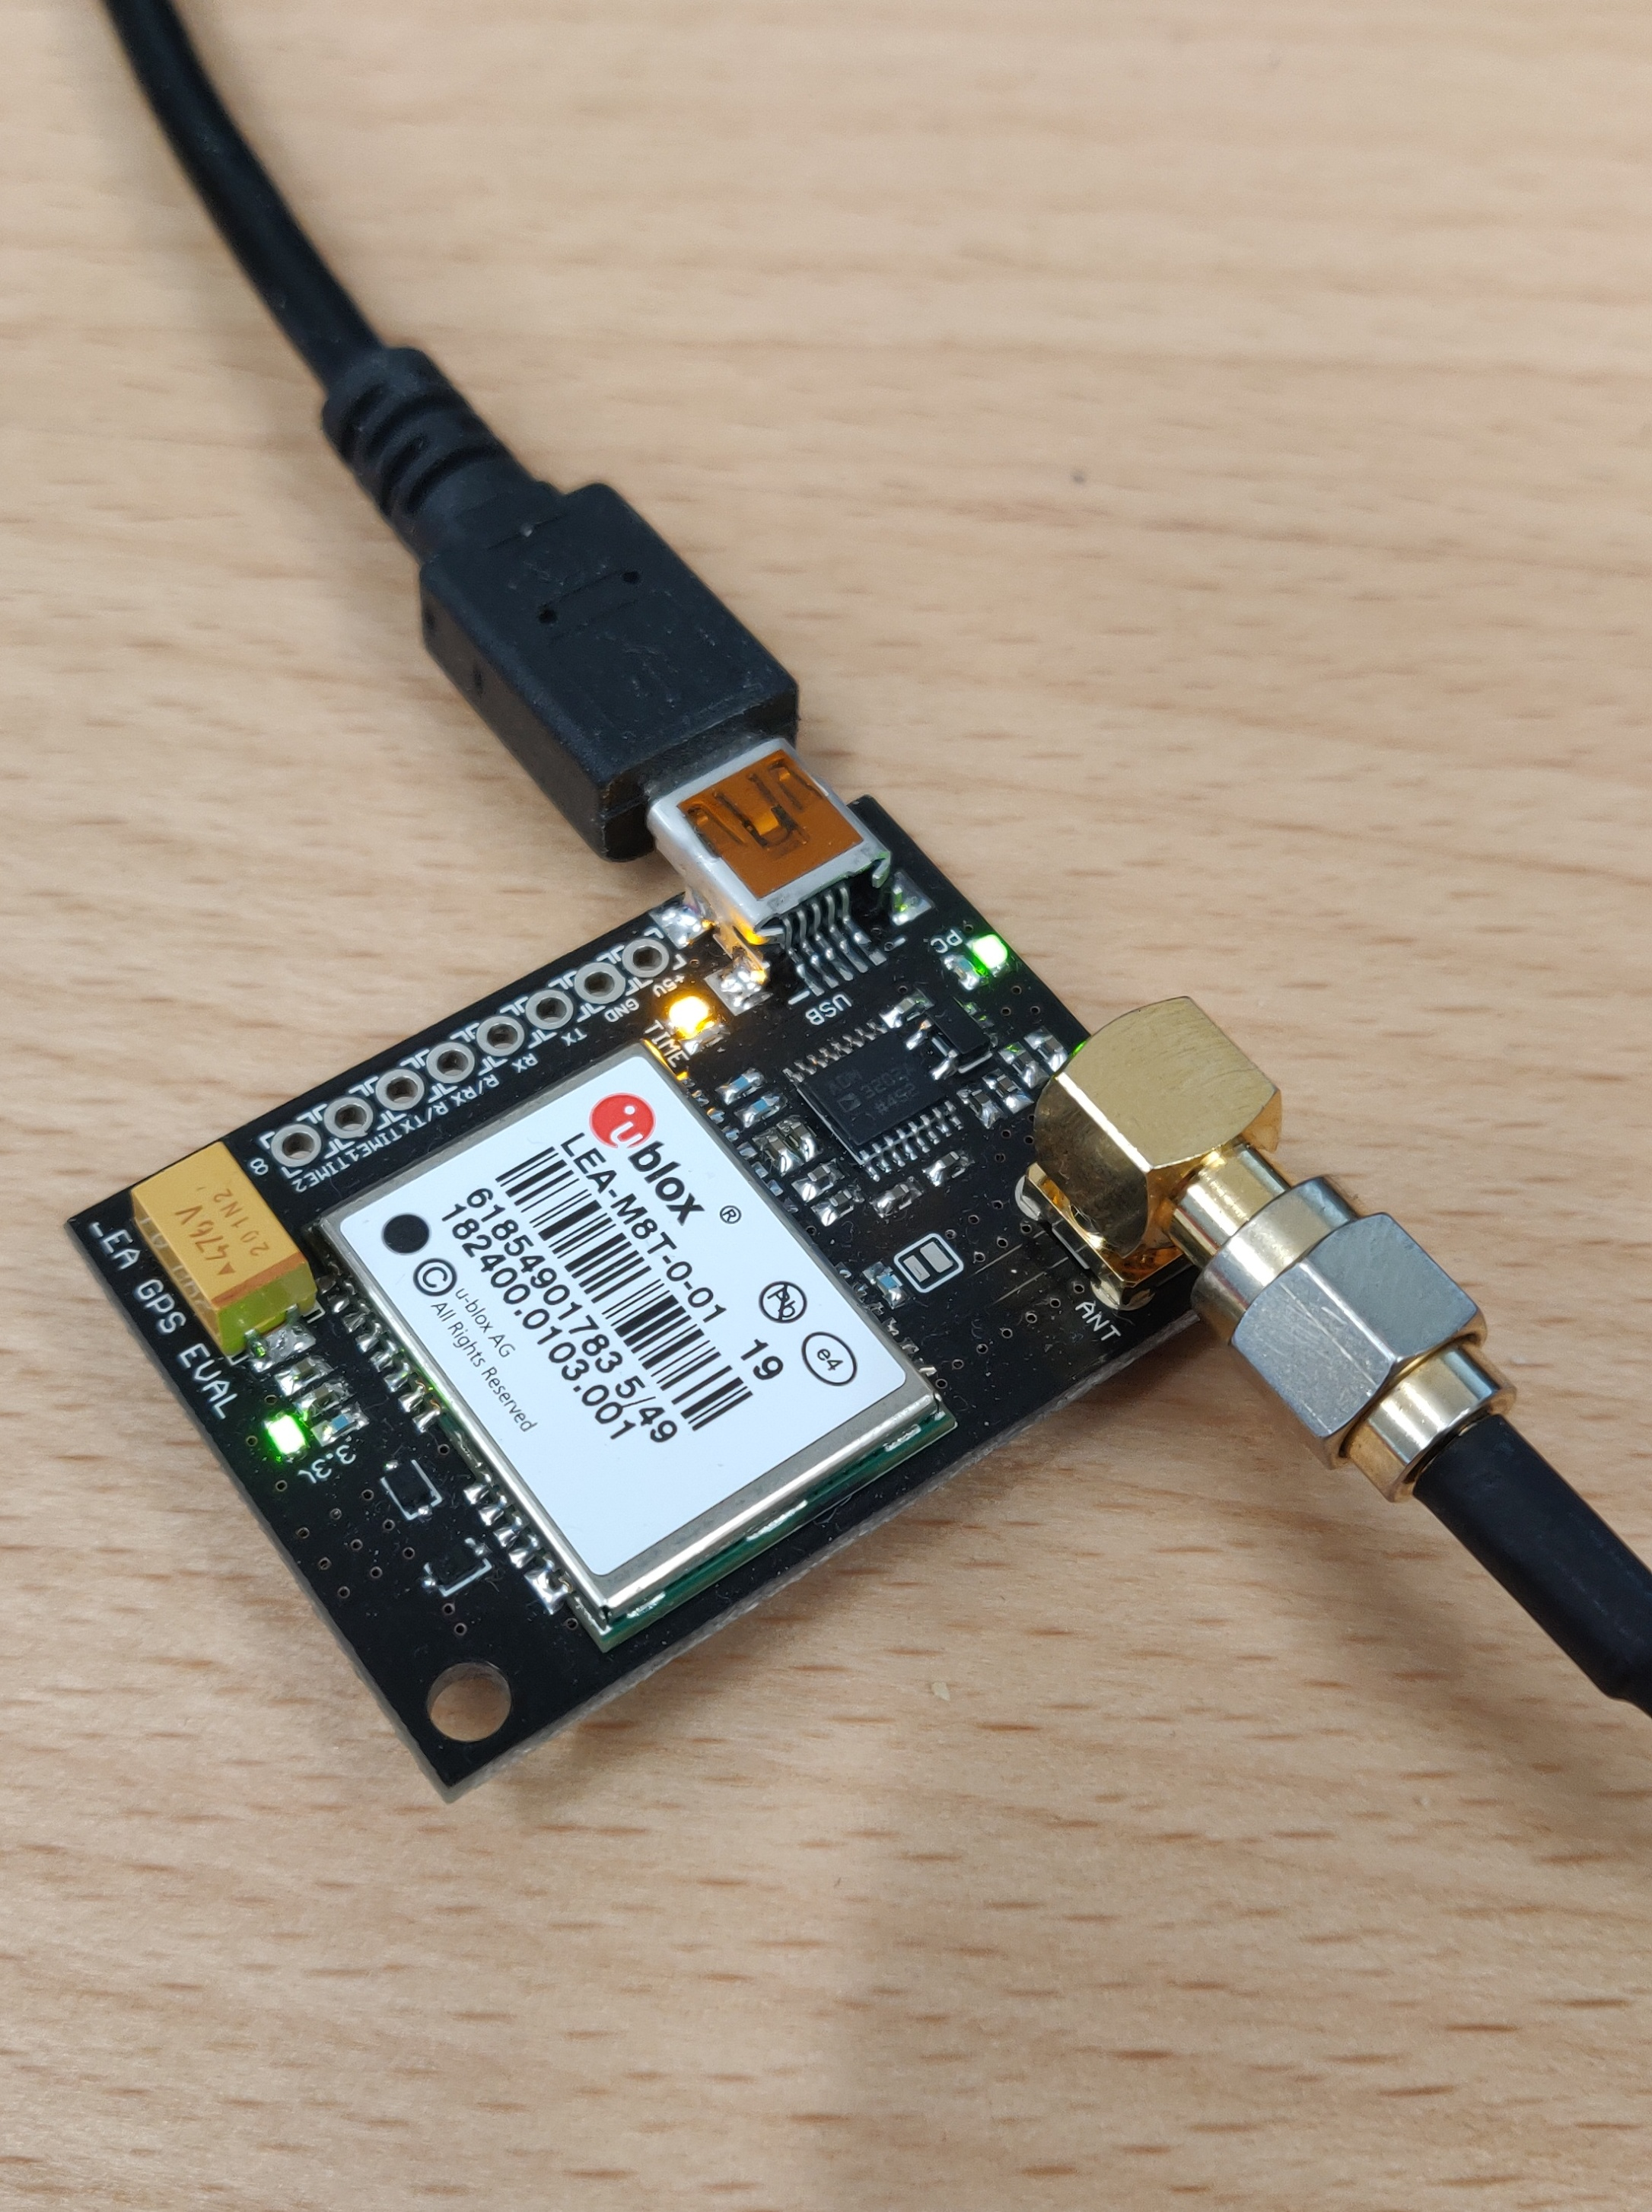
\includegraphics[scale=0.05]{Implementation/Images/lea-m8t.jpg}
            \caption{The Ublox LEA-M8T multi-GNSS receiver}
            \label{fig:lea-m8t}
        \end{figure}
        
    \subsection{IMC log}
        %output log from rtklib doesn't handle IMU
        While the UBX log and live serial device is great for testing both the RTKLIB task and the measurement step of the EKF, it does not contain any IMU measurements, and consequently the dynamics of the prediction step is not properly tested. Testing and tuning the full EKF directly on the hardware is impractical as it can only be updated by the somewhat lengthy process of cross-compilation. However, DUNE has the ability to log any of the message types on the IMC bus and replay it on any other DUNE system. In other words, replaying the log on a computer, the system will virtually behave as if running with the full hardware package. This is invaluable when tuning the Kalman filter as DUNE can be updated directly and efficiently, there will be no unexpected problems related to real world testing and estimates can easily be compared to a reference.